\newcommand{\svrname}{Dr John Fawcett}
\newcommand{\jkfside}{oneside}
\newcommand{\jkfhanded}{right}

\newcommand{\studentname}{Harry Langford}
\newcommand{\studentemail}{hjel2@cam.ac.uk}

\documentclass[10pt,\jkfside,a4paper]{article}

% DO NOT add \usepackage commands here.  Place any custom commands
% into your SV work files.  Anything in the template directory is
% likely to be overwritten!

\usepackage{fancyhdr}

\usepackage{lastpage}       % ``n of m'' page numbering
\usepackage{lscape}         % Makes landscape easier

\usepackage{verbatim}       % Verbatim blocks
\usepackage{listings}       % Source code listings
\usepackage{epsfig}         % Embed encapsulated postscript
\usepackage{array}          % Array environment
\usepackage{qrcode}         % QR codes
\usepackage{enumitem}       % Required by Tom Johnson's exam question header

\usepackage{hhline}         % Horizontal lines in tables
\usepackage{siunitx}        % Correct spacing of units
\usepackage{amsmath}        % American Mathematical Society
\usepackage{amssymb}        % Maths symbols
\usepackage{amsthm}         % Theorems

\usepackage{ifthen}         % Conditional processing in tex

\usepackage[top=3cm,
            bottom=3cm,
            inner=2cm,
            outer=5cm]{geometry}

% PDF metadata + URL formatting
\usepackage[
            pdfauthor={\studentname},
            pdftitle={\svcourse, SV \svnumber},
            pdfsubject={},
            pdfkeywords={9d2547b00aba40b58fa0378774f72ee6},
            pdfproducer={},
            pdfcreator={},
            hidelinks]{hyperref}


% DO NOT add \usepackage commands here.  Place any custom commands
% into your SV work files.  Anything in the template directory is
% likely to be overwritten!

\usepackage{fancyhdr}

\usepackage{lastpage}       % ``n of m'' page numbering
\usepackage{lscape}         % Makes landscape easier

\usepackage{verbatim}       % Verbatim blocks
\usepackage{listings}       % Source code listings
\usepackage{graphicx}
\usepackage{float}
\usepackage{epsfig}         % Embed encapsulated postscript
\usepackage{array}          % Array environment
\usepackage{qrcode}         % QR codes
\usepackage{enumitem}       % Required by Tom Johnson's exam question header

\usepackage{hhline}         % Horizontal lines in tables
\usepackage{siunitx}        % Correct spacing of units
\usepackage{amsmath}        % American Mathematical Society
\usepackage{amssymb}        % Maths symbols
\usepackage{amsthm}         % Theorems

\usepackage{ifthen}         % Conditional processing in tex

\usepackage[top=3cm,
            bottom=3cm,
            inner=2cm,
            outer=5cm]{geometry}

% PDF metadata + URL formatting
\usepackage[
            pdfauthor={\studentname},
            pdftitle={\svcourse, SV \svnumber},
            pdfsubject={},
            pdfkeywords={9d2547b00aba40b58fa0378774f72ee6},
            pdfproducer={},
            pdfcreator={},
            hidelinks]{hyperref}

\renewcommand{\headrulewidth}{0.4pt}
\renewcommand{\footrulewidth}{0.4pt}
\fancyheadoffset[LO,LE,RO,RE]{0pt}
\fancyfootoffset[LO,LE,RO,RE]{0pt}
\pagestyle{fancy}
\fancyhead{}
\fancyhead[LO,RE]{{\bfseries \studentname}\\\studentemail}
\fancyhead[RO,LE]{{\bfseries \svcourse, SV~\svnumber}\\\svdate\ \svtime, \svvenue}
\fancyfoot{}
\fancyfoot[LO,RE]{For: \svrname}
\fancyfoot[RO,LE]{\today\hspace{1cm}\thepage\ / \pageref{LastPage}}
\fancyfoot[C]{\qrcode[height=0.8cm]{\svuploadkey}}
\setlength{\headheight}{22.55pt}


\ifthenelse{\equal{\jkfside}{oneside}}{

 \ifthenelse{\equal{\jkfhanded}{left}}{
  % 1. Left-handed marker, one-sided printing or e-marking, use oneside and...
  \evensidemargin=\oddsidemargin
  \oddsidemargin=73pt
  \setlength{\marginparwidth}{111pt}
  \setlength{\marginparsep}{-\marginparsep}
  \addtolength{\marginparsep}{-\textwidth}
  \addtolength{\marginparsep}{-\marginparwidth}
 }{
  % 2. Right-handed marker, one-sided printing or e-marking, use oneside.
  \setlength{\marginparwidth}{111pt}
 }

}{
 % 3. Alternating margins, two-sided printing, use twoside.
}


\setlength{\parindent}{0em}
\addtolength{\parskip}{1ex}

% Exam question headings, labels and sensible layout (courtesy of Tom Johnson)
\setlist{parsep=\parskip, listparindent=\parindent}
\newcommand{\examhead}[3]{\section{#1 Paper #2 Question #3}}
\newenvironment{examquestion}[3]{
\examhead{#1}{#2}{#3}\setlist[enumerate, 1]{label=(\alph*)}\setlist[enumerate, 2]{label=(\roman*)}
\marginpar{\href{https://www.cl.cam.ac.uk/teaching/exams/pastpapers/y#1p#2q#3.pdf}{\qrcode{https://www.cl.cam.ac.uk/teaching/exams/pastpapers/y#1p#2q#3.pdf}}}
\marginpar{\footnotesize \href{https://www.cl.cam.ac.uk/teaching/exams/pastpapers/y#1p#2q#3.pdf}{https://www.cl.cam.ac.uk/\\teaching/exams/pastpapers/\\y#1p#2q#3.pdf}}
}{}


\fancyhead[RO,LE]{{\bfseries NST Maths, SV~12}\\05-02-22\ 12:00, Video Link}

\usepackage{physics}
\usepackage{graphicx}
\graphicspath{ {./images/} }

\begin{document}

\begin{enumerate}

\setcounter{enumi}{13}

\item 
Since $a \geq 0$, we know that $x^{2} + y^{2} + a^2 \geq 0$.
\begin{equation}
\begin{split}
h(x, y) &= \frac{a(x + y)}{x^{2} + y^{2} + a^2} \\
\left(\pdv{h}{x}\right)_y &= \frac{a((x^{2} + y^{2} + a^2) - 2x(x + y))}{(x^{2} + y^{2} + a^2)^2} \\
\left(\pdv{h}{x}\right)_y &= \frac{a(y^{2} - 2xy - x^{2} + a^2)}{(x^{2} + y^{2} + a^2)^2} \\
0 &= \frac{a(y^{2} - 2xy - x^{2} + a^2)}{(x^{2} + y^{2} + a^2)^2} \\
0 &= a(y^{2} - 2xy - x^{2} + a^2) \\
0 &= y^{2} - 2xy - x^{2} + a^2 \\
\end{split}
\end{equation}

\begin{equation}
\begin{split}
\left(\pdv{h}{y}\right)_x &= \frac{a((x^{2} + y^{2} + a^2) - 2y(x + y))}{(x^{2} + y^{2} + a^2)^2} \\
\left(\pdv{h}{y}\right)_x &= \frac{a(x^{2} - 2xy - y^{2} + a^2)}{(x^{2} + y^{2} + a^2)^2} \\
0 &= a(x^{2} - 2xy - y^{2} + a^2) \\
0 &= x^{2} - 2xy - y^{2} + a^2 \\
\end{split}
\end{equation}

Since at any stationary point, both $\left(\pdv{h}{x}\right)_y = 0$ and $\left(\pdv{h}{y}\right)_x = 0$, 
they must be equal to each other.

\begin{equation}
\begin{split}
x^{2} - 2xy - y^{2} + a^2 &= y^{2} - 2xy - x^{2} + a^2 \\
x^{2} - y^{2} &= y^{2} - x^{2} \\
2x^{2} &= 2y^{2} \\
x^{2} &= y^{2} \\
\end{split}
\end{equation}
\begin{equation}
\begin{split}
0 &= x^{2} - 2xy - y^{2} + a^2 \\
0 &= a^2 - 2xy + (x^{2} - y^{2} \\
0 &= a^2 - 2xy \\
xy &= \frac{a^2}{2} \\
\pm x^{2} &= \frac{a^2}{2} \\
\end{split}
\end{equation}
Since $a \in \mathbb{R}$, $a^2$ must be a positive number and so $\pm x^{2}$ must be positive. \\
This means that:
\begin{equation}
\begin{split}
x^{2} &= \frac{a^2}{2} \\
x &= \pm \frac{a}{\sqrt{2}} \\
y &= \pm \frac{a}{\sqrt{2}} \\
\end{split}
\end{equation}

For a point to be a maximum or a minimum: $h_{xx}h_{yy} > h^2_{xy}$ and $h_{xx} > 0$ and $h_{yy} > 0$.

\begin{equation}
\begin{split}
\left(\pdv{h}{x}\right)_y &= \frac{a(y^{2} - 2xy - x^{2} + a^2)}{(x^{2} + y^{2} + a^2)^2} \\
\left(\pdv[2]{h}{x}\right)_y &= \frac{a((-2y - 2x)(x^{2} + y^{2} + a^2) - 4x(y^{2} - 2xy - x^{2} + a^2))}{(x^{2} + y^{2} + a^2)^3} \\
\left(\pdv[2]{h}{x}\right)_y &= \frac{a(-2x^{2}y - 2x^3 - 2y^3 - 2xy^{2} - 2a^2y - 2a^2x - 4xy^{2} + 8x^{2}y + 4x^3 - 4a^2x)}{(x^{2} + y^{2} + a^2)^3} \\
\left(\pdv[2]{h}{x}\right)_y &= \frac{a(6x^{2}y + 2x^3 - 2y^3 - 6xy^{2} - 2a^2y - 6a^2x)}{(x^{2} + y^{2} + a^2)^3} \\
\left(\pdv{h}{y}\right)_x &= \frac{a(x^{2} - 2xy - y^{2} + a^2)}{(x^{2} + y^{2} + a^2)^2} \\
\left(\pdv[2]{h}{y}\right)_x &= \frac{a(6xy^{2} + 2y^3 - 2x^3 - 6x^{2}y - 2a^2x - 6a^2y)}{(x^{2} + y^{2} + a^2)^3} \\
\left(\pdv[2]{h}{x}{y}\right) &= \frac{a((2y - 2x)(x^{2} + y^{2} + a^2) - 4y(y^{2} - 2xy - x^{2} + a^2))}{(x^{2} + y^{2} + a^2)^3} \\
\left(\pdv[2]{h}{x}{y}\right) &= \frac{a(6x^{2}y - 2y^3 - 2x^3 + 6xy^{2} - 2a^2x - 2a^2y)}{(x^{2} + y^{2} + a^2)^3} \\
\end{split}
\end{equation}

There are four stationary points which we must establish the type of: 
$(\frac{a}{\sqrt{2}}, \frac{a}{\sqrt{2}})$, $(\frac{a}{\sqrt{2}}, -\frac{a}{\sqrt{2}})$, $(-\frac{a}{\sqrt{2}}, \frac{a}{\sqrt{2}})$, 
$(-\frac{a}{\sqrt{2}}, -\frac{a}{\sqrt{2}})$

At $(\frac{a}{\sqrt{2}}, \frac{a}{\sqrt{2}})$:
\begin{equation}
\begin{split}
\left(\pdv[2]{h}{x}\right)_y &= \frac{a(- \sqrt{2}a^3 - 3\sqrt{2}a^3)}{(\frac{a^2}{2} + \frac{a^2}{2} + a^2)^3} \\
\left(\pdv[2]{h}{x}\right)_y &= \frac{- 4\sqrt{2}a^4}{8a^6} \\
\left(\pdv[2]{h}{x}\right)_y &= -\frac{\sqrt{2}}{2a^2} \\
\left(\pdv[2]{h}{y}\right)_x &= -\frac{\sqrt{2}}{2a^2} \\
\left(\pdv[2]{h}{x}{y}\right) &= 0 \\
\end{split}
\end{equation}
Since both $h_{xx} < 0$ and $h_{yy} < 0$ and $h_{xx}h_{yy} = \frac{2}{4a^4} > 0 = h_{xy}$. This is a maximum.

At $(\frac{a}{\sqrt{2}}, -\frac{a}{\sqrt{2}})$:
\begin{equation}
\begin{split}
\left(\pdv[2]{h}{x}\right)_y &= -\frac{\sqrt{2}}{2a^2} \\
\left(\pdv[2]{h}{y}\right)_x &= \frac{\sqrt{2}}{2a^2} \\
\end{split}
\end{equation}
Since $h_{xx}$ and $h_{yy}$ have different signs, we know there cannot be a maxima or minima at this point and so 
will not investigate further.

At $(-\frac{a}{\sqrt{2}}, \frac{a}{\sqrt{2}})$:
\begin{equation}
\begin{split}
\left(\pdv[2]{h}{x}\right)_y &= -\frac{\sqrt{2}}{2a^2} \\
\left(\pdv[2]{h}{y}\right)_x &= \frac{\sqrt{2}}{2a^2} \\
\end{split}
\end{equation}
Since $h_{xx}$ and $h_{yy}$ have different signs, we know there cannot be a maxima or minima at this point and so 
will not investigate further.

At $(-\frac{a}{\sqrt{2}}, -\frac{a}{\sqrt{2}})$:
\begin{equation}
\begin{split}
\left(\pdv[2]{h}{x}\right)_y &= \frac{\sqrt{2}}{2a^2} \\
\left(\pdv[2]{h}{y}\right)_x &= \frac{\sqrt{2}}{2a^2} \\
\left(\pdv[2]{h}{x}{y}\right) &= 0 \\
\end{split}
\end{equation}
Since both $h_{xx} > 0$ and $h_{yy} > 0$ and $h_{xx}h_{yy} = \frac{2}{4a^4} > 0 = h_{xy}$. This is a minimum.

So the maximum is at $(\frac{a}{\sqrt{2}}, \frac{a}{\sqrt{2}})$ and the minimum is at $(-\frac{a}{\sqrt{2}}, -\frac{a}{\sqrt{2}})$.

At the maximum: 
\begin{equation}
\begin{split}
h(\frac{a}{\sqrt{2}}, \frac{a}{\sqrt{2}}) &= \frac{a\left(\frac{a}{\sqrt{2}} + \frac{a}{\sqrt{2}}\right)}{\left(\frac{a}{\sqrt{2}}\right)^2 + \left(\frac{a}{\sqrt{2}}\right)^2 + a^2 } \\
h(\frac{a}{\sqrt{2}}, \frac{a}{\sqrt{2}}) &= \frac{a\left(\sqrt{2}a\right)}{\frac{a^2}{2} + \frac{a^2}{2} + a^2 } \\
h(\frac{a}{\sqrt{2}}, \frac{a}{\sqrt{2}}) &= \frac{\sqrt{2}a^2}{2a^2} \\
h(\frac{a}{\sqrt{2}}, \frac{a}{\sqrt{2}}) &= \frac{1}{\sqrt{2}} \\
\end{split}
\end{equation}

So the maximum height is $\frac{1}{\sqrt{2}}$.

At the minimum:
\begin{equation}
\begin{split}
h(-\frac{a}{\sqrt{2}}, -\frac{a}{\sqrt{2}}) &= \frac{a\left(-\frac{a}{\sqrt{2}} - \frac{a}{\sqrt{2}}\right)}{\left(-\frac{a}{\sqrt{2}}\right)^2 + \left(-\frac{a}{\sqrt{2}}\right)^2 + a^2 } \\
h(-\frac{a}{\sqrt{2}}, -\frac{a}{\sqrt{2}}) &= \frac{a\left(-\sqrt{2}a\right)}{\frac{a^2}{2} + \frac{a^2}{2} + a^2 } \\
h(-\frac{a}{\sqrt{2}}, -\frac{a}{\sqrt{2}}) &= \frac{-\sqrt{2}a^2}{2a^2} \\
h(-\frac{a}{\sqrt{2}}, -\frac{a}{\sqrt{2}}) &= -\frac{1}{\sqrt{2}} \\
\end{split}
\end{equation}

So the minimum height is $-\frac{1}{\sqrt{2}}$.

\begin{center}
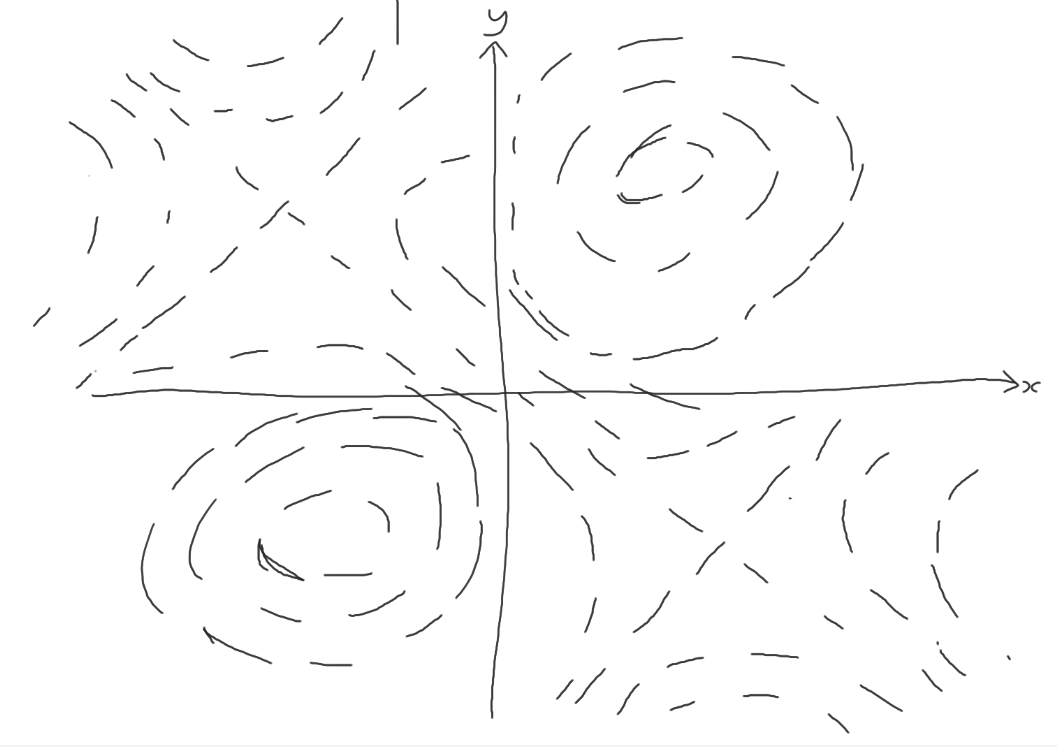
\includegraphics[width=100mm]{sv12sketch2}
\end{center}

\item 
\begin{enumerate}

\item 
\begin{equation}
\begin{split}
z &= (x^{2} - y^{2})e^{- x^{2} - y^{2}} \\
\left(\pdv{z}{x}\right)_y &= 2xe^{-x^{2} - y^{2}} - 2x(x^{2} - y^{2})e^{-x^{2} - y^{2}} \\
0 &= 2x(y^{2} - x^{2} + 1)e^{-x^{2} - y^{2}} \\
0 &= x(y^{2} + 1 - x^{2}) \\
\left(\pdv{z}{y}\right)_x &= -2ye^{-x^{2} - y^{2}} - 2y(x^{2} - y^{2})e^{-x^{2} - y^{2}} \\
0 &= -2y(x^{2} - y^{2} + 1)e^{-x^{2} - y^{2}} \\
0 &= y(x^{2} - y^{2} + 1) \\
\end{split}
\end{equation}

Assume that there is a stationary point with $x \neq 0, y \neq 0$.

\begin{equation}
\begin{split}
y^{2} - x^{2} + 1 &= 0 \\
x^{2} - y^{2} + 1 &= 0 \\
y^{2} - x^{2} + 1 x^{2} - y^{2} + 1 &= 0 \\
2 &= 0 \\
\end{split}
\end{equation}
This is absurd. So there is no stationary point such that $x \neq 0$ and $y \neq 0$.

Take $x = 0$:
\begin{equation}
\begin{split}
0 &= y(x^{2} - y^{2} + 1) \\
y = 0 &\vee 1 - y^{2} = 0 \\
y = 0 &\vee y = 1 \vee y = -1 \\
\end{split}
\end{equation}

Take $y = 0$:
\begin{equation}
\begin{split}
0 &= x(y^{2} - x^{2} + 1) \\
x = 0 &\vee 1 - y^{2} = 0 \\
x = 0 &\vee x = 1 \vee x = -1 \\
\end{split}
\end{equation}

So the stationary points are at:\\
$(0, 0), (0, 1), (0, -1), (-1, 0), (1, 0)$

\item Moving along the contour $z = 0$ satisfies the equation:
\begin{equation}
\begin{split}
0 &= (x^{2} - y^{2})e^{-x^{2} - y^{2}} \\
0 &= x^{2} - y^{2} \\
x &= \pm y \\
\end{split}
\end{equation}

Using this we can see that $(0, 0)$ lies on the contour $z = 0$ and so $(0, 0)$ must be 
a saddle point.

\begin{equation}
\begin{split}
\left(\pdv{z}{x}\right)_y &= 2xe^{-x^{2} - y^{2}} - 2x(x^{2} - y^{2})e^{-x^{2} - y^{2}} \\
\left(\pdv{z}{x}\right)_y &= (2x - 2x^3 + 2xy^{2})e^{-x^{2} - y^{2}} \\
\left(\pdv[2]{z}{x}\right)_y &= (2 - 6x^{2} + 2y^{2} - 4x^{2} + 4x^4 - 4x^{2}y^{2})e^{-x^{2} - y^{2}} \\
\left(\pdv[2]{z}{x}\right)_y &= (2 - 10x^{2} + 2y^{2} + 4x^4 - 4x^{2}y^{2})e^{-x^{2} - y^{2}} \\
\left(\pdv{z}{y}\right)_x &= -2ye^{-x^{2} - y^{2}} - 2y(x^{2} - y^{2})e^{-x^{2} - y^{2}} \\
\left(\pdv{z}{y}\right)_x &= (-2y - 2x^{2}y + 2y^3)e^{-x^{2} - y^{2}} \\
\left(\pdv[2]{z}{y}\right)_x &= (-2 - 2x^{2} + 6y^{2} + 4y^{2} + 4x^{2}y^{2} - 4y^4)e^{-x^{2} - y^{2}} \\
\left(\pdv[2]{z}{y}\right)_x &= (-2 - 2x^{2} + 10y^{2} + 4x^{2}y^{2} - 4y^4)e^{-x^{2} - y^{2}} \\
\left(\pdv[2]{z}{x}{y}\right) &= 4xy(x^{2} - y^{2})e^{-x^{2} - y^{2}} \\
\end{split}
\end{equation}

At $(1, 0)$:
\begin{equation}
\begin{split}
\left(\pdv[2]{z}{x}\right)_y &= -4e^{-1} \\
\left(\pdv[2]{z}{y}\right) &= -4e^{-1} \\
\left(\pdv[2]{z}{x}{y}\right) &= 0 \\
\end{split}
\end{equation}
So $z_{xx} < 0$, $z_{yy} < 0$ and $z_{xx}z_{yy} = 16e^{-1} > f^2_{xy}$.\\
So there is a maximum at $(1, 0)$.

At $(-1, 0)$:
\begin{equation}
\begin{split}
\left(\pdv[2]{z}{x}\right)_y &= -4e^{-1} \\
\left(\pdv[2]{z}{y}\right) &= -4e^{-1} \\
\left(\pdv[2]{z}{x}{y}\right) &= 0 \\
\end{split}
\end{equation}
So $z_{xx} < 0$, $z_{yy} < 0$ and $z_{xx}z_{yy} = 16e^{-1} > f^2_{xy}$.\\
So there is a maximum at $(-1, 0)$.

At $(0, 1)$:
\begin{equation}
\begin{split}
\left(\pdv[2]{z}{x}\right)_y &= 4e^{-1} \\
\left(\pdv[2]{z}{y}\right) &= 4e^{-1} \\
\left(\pdv[2]{z}{x}{y}\right) &= 0 \\
\end{split}
\end{equation}
So $z_{xx} > 0$, $z_{yy} > 0$ and $z_{xx}z_{yy} = 16e^{-1} > f^2_{xy}$.\\
So there is a minimum at $(0, 1)$.

At $(0, -1)$:
\begin{equation}
\begin{split}
\left(\pdv[2]{z}{x}\right)_y &= 4e^{-1} \\
\left(\pdv[2]{z}{y}\right) &= 4e^{-1} \\
\left(\pdv[2]{z}{x}{y}\right) &= 0 \\
\end{split}
\end{equation}
So $z_{xx} > 0$, $z_{yy} > 0$ and $z_{xx}z_{yy} = 16e^{-1} > f^2_{xy}$.\\
So there is a minimum at $(0, -1)$.

\begin{center}
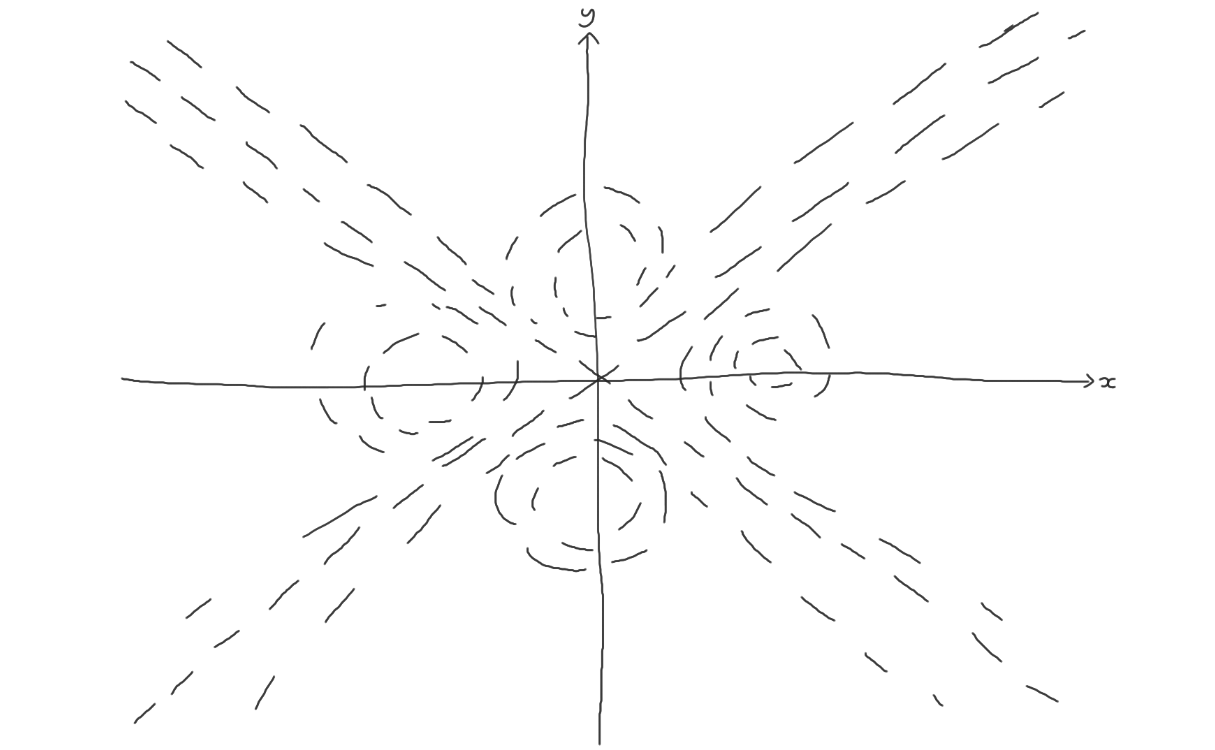
\includegraphics[width=100mm]{sv12sketch}
\end{center}

\end{enumerate}

\item
\begin{enumerate}

\item 
\begin{equation}
\begin{split}
f &= \frac{1}{x^{2} + y^{2} + 1} \\
\left(\pdv{f}{x}\right)_y &= \frac{-2x}{(x^{2} + y^{2} + 1)^2} \\
\left(\pdv[2]{f}{x}\right)_y &= \frac{2x^{2} - 2y^{2} - 2}{(x^{2} + y^{2} + 1)^3} \\
\left(\pdv[2]{f}{x}{y}\right) &= \frac{8xy}{(x^{2} + y^{2} + 1)^3} \\
\left(\pdv{f}{y}\right)_x &= \frac{-2y}{(x^{2} + y^{2} + 1)^2} \\
\left(\pdv[2]{f}{x}\right)_y &= \frac{2y^{2} - 2x^{2} - 2}{(x^{2} + y^{2} + 1)^3} \\
\end{split}
\end{equation}

At any stationary point for the function $f$, $f_x = 0$ and $f_y = 0$:
\begin{equation}
\begin{split}
\left(\pdv{f}{x}\right)_y &= 0 \\
\frac{-2x}{(x^{2} + y^{2} + 1)^2} &= 0 \\
-2x &= 0 \\
x &= 0 \\
\end{split}
\end{equation}
\begin{equation}
\begin{split}
\left(\pdv{f}{x}\right)_y &= 0 \\
\frac{-2y}{(x^{2} + y^{2} + 1)^2} &= 0 \\
-2y &= 0 \\
y &= 0 \\
\end{split}
\end{equation}
So the only stationary point for the function $f$ is at $(0, 0)$.

At $(0, 0)$:
\begin{equation}
\begin{split}
\left(\pdv[2]{f}{x}\right)_y &= -2 \\
\left(\pdv[2]{f}{y}\right)_x &= -2 \\
\left(\pdv[2]{f}{x}{y}\right) &= 0 \\
\end{split}
\end{equation}
So $f_{xx} < 0$, $f_{yy} < 0$ and $f_{xx}f_{yy} > f^2_{xy}$.

This means that there is a maximum at $(0, 0)$.

\item 
\begin{equation}
\begin{split}
f &= \sin x \sin y \\
\left(\pdv{f}{x}\right)_y &= \cos x \sin y \\
\left(\pdv[2]{f}{x}\right)_y &= - \sin x \sin y \\
\left(\pdv{f}{y}\right)_x &= \sin x \cos y \\
\left(\pdv[2]{f}{y}\right)_x &= - \sin x \sin y \\
\left(\pdv[2]{f}{x}{y}\right) &= \cos x \cos y \\
\end{split}
\end{equation}

At any stationary point of the function $f$, $f_x = f_y = 0$.
\begin{equation}
\begin{split}
0 &= \cos x \sin y = \sin x \cos y \\
\cos x &= 0 \wedge \cos y = 0 \vee \sin y = 0 \wedge \sin x = 0 \\
x &= \frac{\pi}{2} \wedge y = \frac{\pi}{2} \\
\end{split}
\end{equation}
So the only stationary point of the function in the range $x, y \in (0, \pi)$ is 
$\left(\frac{\pi}{2}, \frac{\pi}{2}\right)$.

At $(\frac{\pi}{2}, \frac{\pi}{2})$, the partial derivatives are:
\begin{equation}
\begin{split}
\left(\pdv[2]{f}{x}\right)_y &= -1 \\
\left(\pdv[2]{f}{y}\right)_x &= -1 \\
\left(\pdv[2]{f}{x}{y}\right) &= 0 \\
\end{split}
\end{equation}
So $f_{xx}f_{yy} = 1 > f^2_{xy}$.

So this point is a maximum:\\
The only stationary point on the curve in the range given is $\left(\frac{\pi}{2}, \frac{\pi}{2}\right)$ 
and is a maximum.

\item 
\begin{equation}
\begin{split}
f &= (xy - y)e^{2x - x^{2} - y^{2}} \\
\left(\pdv{f}{x}\right)_y &= y(- 2x^{2} + 4x - 1)e^{2x - x^{2} - y^{2}} \\
\left(\pdv[2]{f}{x}\right)_y &= y(4x^3 - 12x^{2} + 6x + 2)e^{2x - x^{2} - y^{2}} \\
\left(\pdv[2]{f}{x}{y}\right) &= (4x^{2}y^{2} - 8xy^{2} + 2y^{2} - 2x^{2} + 4x - 1)e^{2x - x^{2} - y^{2}}\\
\left(\pdv{f}{y}\right)_x &= (x - 1)e^{2x - x^{2} - y^{2}} - 2y(xy - y)e^{2x - x^{2} - y^{2}} \\
\left(\pdv{f}{y}\right)_x &= (x - 1 - 2xy^{2} + 2y^{2})e^{2x - x^{2} - y^{2}} \\
\left(\pdv[2]{f}{y}\right)_x &= (4y - 4xy)e^{2x - x^{2} - y^{2}} - 2y(x - 1 - 2xy^{2} + 2y^{2})e^{2x - x^{2} - y^{2}} \\
\left(\pdv[2]{f}{y}\right)_x &= y(6 - 6x + 4xy^{2} - 4y^{2})e^{2x - x^{2} - y^{2}} \\
\end{split}
\end{equation}

At any stationary point, both $f_x = 0$ and $f_y = 0$.

\begin{equation}
\begin{split}
\left(\pdv{f}{x}\right)_y &= 0 \\
y(- 2x^{2} + 4x - 1)e^{2x - x^{2} - y^{2}} &= 0 \\
y = 0 \vee 2x^{2} - 4x + 1 &= 0 \\
y = 0 \vee x = 1 + \frac{\sqrt{2}}{2} \vee x = 1 &- \frac{\sqrt{2}}{2} \\
\end{split}
\end{equation}
\begin{equation}
\begin{split}
\left(\pdv{f}{y}\right)_x &= 0 \\
(x - 1 - 2xy^{2} + 2y^{2})e^{2x - x^{2} - y^{2}} &= 0 \\
x - 1 - 2xy^{2} + 2y^{2} &= 0 \\
\text{For } y = 0 \\
x - 1 &= 0 \\
x &= 1 \\
\text{For } x = 1 + \frac{\sqrt{2}}{2} \\
1 + \frac{\sqrt{2}}{2} - 1 - 2y^{2} - \sqrt{2}y^{2} + y^{2} &= 0 \\
\sqrt{2}y^{2} &= \frac{\sqrt{2}}{2} \\
y &= \pm \frac{\sqrt{2}}{2} \\
\text{For } x = 1 - \frac{\sqrt{2}}{2} \\
1 - \frac{\sqrt{2}}{2} - 1 - 2y^{2} + \sqrt{2}y^{2} + y^{2} &= 0 \\
\sqrt{2}y^{2} &= \frac{\sqrt{2}}{2} \\
y &= \pm \frac{\sqrt{2}}{2} \\
\end{split}
\end{equation}
So there are five stationary points:\\
$(1, 0), (1 - \frac{\sqrt{2}}{2}, \frac{\sqrt{2}}{2}), (1 - \frac{\sqrt{2}}{2}, - \frac{\sqrt{2}}{2}), (1 + \frac{\sqrt{2}}{2}, \frac{\sqrt{2}}{2}), (1 + \frac{\sqrt{2}}{2}, - \frac{\sqrt{2}}{2})$

At (1, 0):
\begin{equation}
\begin{split}
\left(\pdv[2]{f}{x}\right)_y &= y(4x^3 - 12x^{2} + 6x + 2)e^{2x - x^{2} - y^{2}} \\
\left(\pdv[2]{f}{x}\right)_y &= 0 \\
\left(\pdv[2]{f}{y}\right)_x &= y(6 - 6x + 4xy^{2} - 4y^{2})e^{2x - x^{2} - y^{2}} \\
\left(\pdv[2]{f}{y}\right)_x &= 0 \\
\left(\pdv[2]{f}{x}{y}\right) &= (4x^{2}y^{2} - 8xy^{2} + 2y^{2} - 2x^{2} + 4x - 1)e^{2x - x^{2} - y^{2}}\\
\left(\pdv[2]{f}{x}{y}\right) &= e \\
\left(\pdv{f}{x}\right)_y \left(\pdv{f}{y}\right)_x &= 0 < \left(\pdv[2]{f}{x}{y}\right) \\
\end{split}
\end{equation}
However, since $\left(\pdv{f}{x}\right)_y = \left(\pdv{f}{y}\right)_x = 0$, we cannot 
claim that they have the opposite side and so cannot tell whether this is a maximum, 
minimum or a saddle point.

At $(1 - \frac{\sqrt{2}}{2}, \frac{\sqrt{2}}{2})$:
\begin{equation}
\begin{split}
\left(\pdv[2]{f}{x}\right)_y &= y(4x^3 - 12x^{2} + 6x + 2)e^{2x - x^{2} - y^{2}} \\
\left(\pdv[2]{f}{x}\right)_y &= 2 \\
\left(\pdv[2]{f}{y}\right)_x &= y(6 - 6x + 4xy^{2} - 4y^{2})e^{2x - x^{2} - y^{2}} \\
\left(\pdv[2]{f}{y}\right)_x &= 2 \\
\left(\pdv[2]{f}{x}{y}\right) &= (4x^{2}y^{2} - 8xy^{2} + 2y^{2} - 2x^{2} + 4x - 1)e^{2x - x^{2} - y^{2}}\\
\left(\pdv[2]{f}{x}{y}\right) &= 0 \\
\left(\pdv{f}{x}\right)_y \left(\pdv{f}{y}\right)_x &= 4 > \left(\pdv[2]{f}{x}{y}\right) \\
\end{split}
\end{equation}

Since both $\left(\pdv[2]{f}{x}\right)_y$ and $\left(\pdv[2]{f}{y}\right)_x$ are positive 
at this value, this must be a minimum. So the function has a minimum at $(1 - \frac{\sqrt{2}}{2}, \frac{\sqrt{2}}{2})$.

At $(1 - \frac{\sqrt{2}}{2}, -\frac{\sqrt{2}}{2})$:
\begin{equation}
\begin{split}
\left(\pdv[2]{f}{x}\right)_y &= y(4x^3 - 12x^{2} + 6x + 2)e^{2x - x^{2} - y^{2}} \\
\left(\pdv[2]{f}{x}\right)_y &= -2 \\
\left(\pdv[2]{f}{y}\right)_x &= y(6 - 6x + 4xy^{2} - 4y^{2})e^{2x - x^{2} - y^{2}} \\
\left(\pdv[2]{f}{y}\right)_x &= -2 \\
\left(\pdv[2]{f}{x}{y}\right) &= (4x^{2}y^{2} - 8xy^{2} + 2y^{2} - 2x^{2} + 4x - 1)e^{2x - x^{2} - y^{2}}\\
\left(\pdv[2]{f}{x}{y}\right) &= 0 \\
\left(\pdv{f}{x}\right)_y \left(\pdv{f}{y}\right)_x &= 4 > \left(\pdv[2]{f}{x}{y}\right) \\
\end{split}
\end{equation}

Since both $\left(\pdv[2]{f}{x}\right)_y$ and $\left(\pdv[2]{f}{y}\right)_x$ are negative 
at this value, this must be a maximum. So the function has a maximum at $(1 - \frac{\sqrt{2}}{2}, -\frac{\sqrt{2}}{2})$.

At $(1 + \frac{\sqrt{2}}{2}, \frac{\sqrt{2}}{2})$:
\begin{equation}
\begin{split}
\left(\pdv[2]{f}{x}\right)_y &= y(4x^3 - 12x^{2} + 6x + 2)e^{2x - x^{2} - y^{2}} \\
\left(\pdv[2]{f}{x}\right)_y &= -2 \\
\left(\pdv[2]{f}{y}\right)_x &= y(6 - 6x + 4xy^{2} - 4y^{2})e^{2x - x^{2} - y^{2}} \\
\left(\pdv[2]{f}{y}\right)_x &= -2 \\
\left(\pdv[2]{f}{x}{y}\right) &= (4x^{2}y^{2} - 8xy^{2} + 2y^{2} - 2x^{2} + 4x - 1)e^{2x - x^{2} - y^{2}}\\
\left(\pdv[2]{f}{x}{y}\right) &= 0 \\
\left(\pdv{f}{x}\right)_y \left(\pdv{f}{y}\right)_x &= 4 > \left(\pdv[2]{f}{x}{y}\right) \\
\end{split}
\end{equation}

Since both $\left(\pdv[2]{f}{x}\right)_y$ and $\left(\pdv[2]{f}{y}\right)_x$ are negative 
at this value, this must be a maximum. So the function has a maximum at $(1 + \frac{\sqrt{2}}{2}, \frac{\sqrt{2}}{2})$.

At $(1 + \frac{\sqrt{2}}{2}, -\frac{\sqrt{2}}{2})$:
\begin{equation}
\begin{split}
\left(\pdv[2]{f}{x}\right)_y &= y(4x^3 - 12x^{2} + 6x + 2)e^{2x - x^{2} - y^{2}} \\
\left(\pdv[2]{f}{x}\right)_y &= 2 \\
\left(\pdv[2]{f}{y}\right)_x &= y(6 - 6x + 4xy^{2} - 4y^{2})e^{2x - x^{2} - y^{2}} \\
\left(\pdv[2]{f}{y}\right)_x &= 2 \\
\left(\pdv[2]{f}{x}{y}\right) &= (4x^{2}y^{2} - 8xy^{2} + 2y^{2} - 2x^{2} + 4x - 1)e^{2x - x^{2} - y^{2}}\\
\left(\pdv[2]{f}{x}{y}\right) &= 0 \\
\left(\pdv{f}{x}\right)_y \left(\pdv{f}{y}\right)_x &= 4 > \left(\pdv[2]{f}{x}{y}\right) \\
\end{split}
\end{equation}

Since both $\left(\pdv[2]{f}{x}\right)_y$ and $\left(\pdv[2]{f}{y}\right)_x$ are positive 
at this value, this must be a minimum. So the function has a minimum at $(1 + \frac{\sqrt{2}}{2}, -\frac{\sqrt{2}}{2})$.

\end{enumerate}

\item 
\begin{enumerate}

\item 
\begin{equation}
\begin{split}
f &= xy^{2} \\
\nabla(f) &= (y^{2}, 2xy) \\
\end{split}
\end{equation}
\begin{equation}
\begin{split}
1 &= x^{2} + y^{2} \\
0 &= x^{2} + y^{2} - 1 \\
g &= x^{2} + y^{2} - 1 \\
\nabla(g) &= (2x, 2y) \\
\end{split}
\end{equation}

\begin{equation}
\begin{split}
y^{2} &= 2\lambda x \\
2xy &= 2 \lambda y \\
x^{2} + y^{2} &= 1 \\
x^{2} + 2\lambda x &= 1 \\
x^{2} + 2\lambda x - 1 &= 0 \\
\end{split}
\end{equation}
\begin{equation}
\begin{split}
x &= \frac{-2\lambda \pm \sqrt{4\lambda^2 + 4}}{2} \\
x &= -\lambda \pm \sqrt{\lambda^2 + 1} \\
2\lambda y &= 2(\lambda \pm \sqrt{\lambda^2 + 1}) y \\
\lambda &= -\lambda \pm \sqrt{\lambda^2 + 1} \vee y = 0\\
2\lambda &= \pm \sqrt{\lambda^2 + 1} \\
4\lambda^2 &= \lambda^2 + 1 \\
3\lambda^2 &= 1 \\
\lambda &= \pm\frac{\sqrt{3}}{3} \\
\end{split}
\end{equation}
\begin{equation}
\begin{split}
2xy &= 2 \lambda y \\
x &= \lambda \\
x &= \pm \frac{\sqrt{3}}{3} \\
y^{2} &= 2\lambda x \\
y^{2} &= 2\lambda^2 \\
y &= \pm\sqrt{2}\lambda \\
y &= \pm\frac{\sqrt{6}}{3} \\
\end{split}
\end{equation}

At $y = 0$, $x = \pm 1$.

So the function $xy^{2}$ subject to the constraint $x^{2} + y^{2} = 1$ has stationary points at:
$(1, 0), (-1, 0), \left(\frac{\sqrt{3}}{3}, \frac{\sqrt{6}}{3}\right), \left(\frac{\sqrt{3}}{3}, -\frac{\sqrt{6}}{3}\right), \left(-\frac{\sqrt{3}}{3}, \frac{\sqrt{6}}{3}\right), \left(-\frac{\sqrt{3}}{3}, -\frac{\sqrt{6}}{3}\right)$

Verification by using the substitution $x = \cos \theta$, $y = \sin \theta$.

\begin{equation}
\begin{split}
f &= xy^2 \\
f &= \cos \theta - \cos^3\theta \\
\dv{f}{\theta} &= -\sin\theta + 3\sin\theta\cos^2\theta \\
0 &= -\sin\theta + 3\sin\theta\cos^2\theta \\
0 &= \sin\theta(3\cos\theta - 1) \\
\end{split}
\end{equation}
So $\sin\theta = 0$ or $3\cos^2\theta = 1$.

At $\sin\theta = 0$:
\begin{equation}
\begin{split}
\sin\theta &= 0 \\
\theta = 0 &\vee \theta = \pi \\
y = 0 \wedge x = -1 &\vee y = 0 \wedge x = 1 \\
\end{split}
\end{equation}
These are stationary points we also found using the lagrangian method.

At $3\cos^2\theta = 1$:
\begin{equation}
\begin{split}
\cos\theta &= \pm\frac{\sqrt{3}}{3} \\
x = \pm\frac{\sqrt{3}}{3}&, y = \pm\frac{\sqrt{6}}{3} \\
\end{split}
\end{equation}
These are the rest of the stationary points we found using the lagrangian method.

So we have found all the same stationary points using the two different methods.

\item
\begin{equation}
\begin{split}
f &= e^{-xy} \\
\nabla(f) &= (-ye^{-xy}, -xe^{-xy}) \\
g &= x^{2} + y^{2} - 1 \\
\nabla(g) &= (2x, 2y) \\
\end{split}
\end{equation}

Using these and the initial constraint we can form three equations and then solve to 
find the stationary points.

\begin{equation}
\begin{split}
-ye^{-xy} &= 2\lambda x \\
-xe^{-xy} &= 2\lambda y \\
x^{2} + y^{2} &= 1 \\
\end{split}
\end{equation}
Note that at $x = 0$, $y$ can be either positive or negative. If we make $x > 0$ for some 
small value, then the value of $-xy$ will become nonzero. So $e^{-xy}$ will increase if $y < 0$ 
and decrease if $y > 0$. The inverse argument holds for making $x < 0$. Since a small change 
in $x$ can increase or decrease $e^{-xy}$ we can conclude that this is not a minimum. So we do 
not need to consider this case.

\begin{equation}
\begin{split}
-ye^{-xy} &= 2\lambda x \\
-\frac{e^{-xy}}{2\lambda} &= \frac{x}{y} \\
-xe^{-xy} &= 2\lambda y \\
-\frac{e^{-xy}}{2\lambda} &= \frac{y}{x} \\
\frac{x}{y} &= \frac{y}{x} \\
x^{2} &= y^{2} \\
x^{2} + y^{2} &= 1 \\ 
x^{2} + x^{2} &= 1 \\
2x^{2} &= 1 \\
x^{2} &= \frac{1}{2} \\
x = \pm\frac{\sqrt{2}}{2}&, y = \pm\frac{\sqrt{2}}{2} \\
\end{split}
\end{equation}

So the function $e^{-xy}$ subject to the constraint $x^{2} + y^{2} = 1$ has stationary points at 
$\left(\frac{\sqrt{2}}{2}, \frac{\sqrt{2}}{2}\right), \left(\frac{\sqrt{2}}{2}, -\frac{\sqrt{2}}{2}\right), \left(-\frac{\sqrt{2}}{2}, \frac{\sqrt{2}}{2}\right), \left(-\frac{\sqrt{2}}{2}, -\frac{\sqrt{2}}{2}\right)$

Informally looking at the value of the function at those points, I can conclude that the 
stationary points at $\left(\frac{\sqrt{2}}{2}, \frac{\sqrt{2}}{2}\right), \left(\frac{\sqrt{2}}{2}, -\frac{\sqrt{2}}{2}\right)$ are maxima 
and those at \\ $\left(-\frac{\sqrt{2}}{2}, \frac{\sqrt{2}}{2}\right), \left(-\frac{\sqrt{2}}{2}, -\frac{\sqrt{2}}{2}\right)$ 
are minima.

Verification using the substition $x = \cos \theta$ and $y = \sin \theta$:

\begin{equation}
\begin{split}
f &= e^{-\frac{1}{2}\sin2\theta} \\
\dv{f}{\theta} &= -\cos2\theta e^{-\frac{1}{2}\sin2\theta} \\
0 &= -\cos2\theta e^{-\frac{1}{2}\sin2\theta} \\
0 &= -\cos2\theta \\
\theta &= \frac{\pi}{4} \vee \frac{3\pi}{4} \vee \frac{5\pi}{4} \vee \frac{7\pi}{4} \\
x = \pm \frac{\sqrt{2}}{2}&, y = \pm \frac{\sqrt{2}}{2} \\
\end{split}
\end{equation}

This is the same result as obtained by the lagrangian method.

\end{enumerate}

\item 
\begin{equation}
\begin{split}
V &= 2x \times 2y \times 2z \\ 
V &= 8xyz \\
\nabla(V) &= (8yz, 8xz, 8xy) \\
g &= \frac{x^{2}}{a^2} + \frac{y^{2}}{b^2} + \frac{z^2}{c^2} - 1 \\
\nabla(g) &= \left(\frac{2x}{a^2}, \frac{2y}{b^2}, \frac{2z}{c^2}\right) \\
\end{split}
\end{equation}

We now form the equations shown below and use these to find the stationary points.
\begin{equation}
\begin{split}
8yz &= \lambda\frac{2x}{a^2} \\
8xz &= \lambda\frac{2y}{b^2} \\
8xy &= \lambda\frac{2z}{c^2} \\
\frac{x^{2}}{a^2} + \frac{y^{2}}{b^2} + \frac{z^2}{c^2} &= 1 \\
\end{split}
\end{equation}

Since we know that $x, y, z$ are distances: they are nonzero and non-negative. This 
means that we know minmuma will occur whenever $x = 0, y = 0, z = 0$ and can 
multiply and divide by $x, y, z$ without worrying about zeros.

\begin{equation}
\begin{split}
y &= \lambda\frac{x}{4a^2z} \\
8xz &= \lambda^2\frac{x}{2a^2b^2z} \\
16a^2b^2z^2 &= \lambda^2 \\
\lambda8x\frac{x}{4a^2z} &= \lambda\frac{2z}{c^2} \\
\frac{2x^{2}}{a^2z} &= \frac{2z}{c^2} \\
c^2x^{2} &= a^2z^2 \\
z^2 &= \frac{c^2x^{2}}{a^2} \\
\end{split}
\end{equation}
\begin{equation}
\begin{split}
16a^2b^2z^2 &= \lambda^2 \\
16a^2b^2\frac{c^2x^{2}}{a^2} &= \lambda^2 \\
x^{2} &= \frac{\lambda^2}{16b^2c^2} \\
z^2 &= \frac{c^2x^{2}}{a^2} \\
z^2 &= \frac{\lambda^2}{16a^2b^2} \\
y^{2} &= \frac{\lambda^2x^{2}}{16a^4z^2} \\
y^{2} &= \frac{\lambda^2}{16a^2c^2} \\
\end{split}
\end{equation}
Now we can substitute our results into the euqation, work out the value for $\lambda$ and 
then substitute it back into the value for $x, y, z$ to work out the maxima.

\begin{equation}
\begin{split}
\frac{x^{2}}{a^2} + \frac{y^{2}}{b^2} + \frac{z^2}{c^2} &= 1 \\
\frac{\lambda}{16a^2b^2c^2} + \frac{\lambda}{16a^2b^2c^2} + \frac{\lambda}{16a^2b^2c^2} &= 1 \\
\end{split}
\end{equation}
\begin{equation}
\begin{split}
3\lambda^2 &= 16a^2b^2c^2 \\
\lambda^2 &= \frac{16a^2b^2c^2}{3} \\
x^{2} &= \frac{\lambda^2}{16b^2c^2} \\
x^{2} &= \frac{16a^2b^2c^2}{48b^2c^2} \\
x^{2} &= \frac{a^2}{3} \\
y^{2} &= \frac{\lambda^2}{16a^2c^2} \\
y^{2} &= \frac{16a^2b^2c^2}{48a^2c^2} \\
y &= \frac{b^2}{3} \\
z^2 &= \frac{\lambda^2}{16a^2b^2} \\
z^2 &= \frac{16a^2b^2c^2}{48a^2b^2} \\
z^2 &= \frac{c^2}{3} \\
\end{split}
\end{equation}
Substituting this back into the equation for Volume gives:
\begin{equation}
\begin{split}
V^2 &= 64 x^{2}y^{2}z^2 \\
V^2 &= \frac{64a^2b^2c^2}{27} \\
V &= \frac{8abc}{\sqrt{27}} \\
\end{split}
\end{equation}
Note that we took the positive root since we know that volume must be greater than zero.

\item 
I will solve the general formula first maximising area when $a + b + c = k$ and then 
will set $k = 2$.
\begin{equation}
\begin{split}
A &= \sqrt{s(s - a)(s - b)(s - c)} \\
\nabla(A) &= \left(-\frac{\sqrt{s(s - b)(s - c)}}{2\sqrt{s - a}}, -\frac{\sqrt{s(s - a)(s - c)}}{2\sqrt{s - b}}, -\frac{\sqrt{s(s - a)(s - b)}}{2\sqrt{s - c}}\right) \\
s &= \frac{1}{2}(a + b + c) \\
0 &= \frac{1}{2}(a + b + c) - s \\
0 &= a + b + c - 2s \\
g &= a + b + c - 2s \\
\nabla(g) &= (1, 1, 1) \\
\end{split}
\end{equation}
Now we have four equations:
\begin{equation}
\begin{split}
\frac{\sqrt{s(s - b)(s - c)}}{\sqrt{s - a}} &= \lambda \\
\frac{\sqrt{s(s - a)(s - c)}}{\sqrt{s - b}} &= \lambda \\
\frac{\sqrt{s(s - a)(s - b)}}{\sqrt{s - c}} &= \lambda \\
a + b + c - 2s &= 0 \\
\end{split}
\end{equation}
Equating them will solve the equation.
\begin{equation}
\begin{split}
-\frac{\sqrt{s(s - b)(s - c)}}{2\sqrt{s - a}} &= -\frac{\sqrt{s(s - a)(s - c)}}{2\sqrt{s - b}} \\
s - b &= s - a \\
a &= b \\
-\frac{\sqrt{s(s - b)(s - c)}}{2\sqrt{s - a}} &= -\frac{\sqrt{s(s - a)(s - b)}}{2\sqrt{s - c}} \\
s - c &= s - a \\
a &= c \\
\end{split}
\end{equation}
So the maximum occurs when $a = b = c$. Since all the side lengths are equal, this is an 
equilateral triangle. So the maximal area of a triangle with total side length $2s$ occurs 
when $a = b = c$ and the triangle is equilateral.

Since $s$ is arbitrary and we have proved this result for perimeter $= 2s$, this result holds for all 
perimeters.

\item 
\begin{equation}
\begin{split}
r &= \sqrt{x^{2} + y^{2} + z^2} \\
\nabla(r) &= \left(\frac{x}{r}, \frac{y}{r}, \frac{z}{r} \right) \\
1 &= \frac{x^{2}}{a^2} + \frac{y^{2}}{b^2} + \frac{z^2}{c^2} \\ 
0 &= \frac{x^{2}}{a^2} + \frac{y^{2}}{b^2} + \frac{z^2}{c^2} - 1 \\ 
g &= \frac{x^{2}}{a^2} + \frac{y^{2}}{b^2} + \frac{z^2}{c^2} - 1 \\ 
\nabla(g) &= \left(\frac{2x}{a^2}, \frac{2y}{b^2}, \frac{2z}{c^2} \right) \\
h &= \ell x + my + nz \\
\nabla(h) &= (\ell, m, n) \\
\end{split}
\end{equation}
\begin{equation}
\begin{split}
\frac{x}{r} &= \lambda \frac{2x}{a^2}  + \mu \ell \\
x &= \frac{\mu r a^2 \ell}{a^2 - 2 r \lambda} \\
\frac{y}{r} &= \lambda \frac{2y}{b^2} + \mu m \\
y &= \frac{\mu r b^2 m}{b^2 - 2 r \lambda} \\
\frac{z}{r} &= \lambda \frac{2z}{c^2} + \mu n \\
z &= \frac{\mu r c^2 n}{c^2 - 2 r \lambda} \\
1 &= \frac{x^{2}}{a^2} + \frac{y^{2}}{b^2} + \frac{z^2}{c^2} \\
0 &= \ell x + my + nz \\
0 &= \ell \left(\frac{\mu r a^2 \ell}{a^2 - 2 r \lambda}\right) + m\left(\frac{\mu r b^2 m}{b^2 - 2 r \lambda}\right) + n\left(\frac{\mu r c^2 n}{c^2 - 2 r \lambda}\right) \\
0 &= \mu r\left(\frac{\ell^2a^2}{a^2 - 2r\lambda} + \frac{m^2b^2}{b^2 - 2r\lambda} + \frac{n^2c^2}{c^2 - 2 r \lambda} \right) \\
\end{split}
\end{equation}

Note that $\mu = 0$ is not a valid solution and that since there are value of $r$ which satisfy the 
constaints which are $> 0$, the maximum value of $r$ is nonzero. So:
\begin{equation}
0 = \frac{\ell^2a^2}{a^2 - 2r\lambda} + \frac{m^2b^2}{b^2 - 2r\lambda} + \frac{n^2c^2}{c^2 - 2 r \lambda} \\
\end{equation}

Consider now $\frac{1}{a^2}$, $\frac{1}{b^2}$ and $\frac{1}{b^2}$:\\
Derived from the equations above:
\begin{equation}
\begin{split}
\frac{1}{a^2} &= \frac{x - \mu r \ell}{2\lambda r x} \\
\frac{1}{b^2} &= \frac{y - \mu r m}{2\lambda r y} \\
\frac{1}{c^2} &= \frac{z - \mu r n}{2\lambda r z} \\
1 &= \frac{x^{2}}{a^2} + \frac{y^{2}}{b^2} + \frac{z^2}{c^2} \\
1 &= \frac{x^{2}(x - \mu r \ell)}{2\lambda r x} + \frac{y^{2}(y - \mu r m)}{2\lambda r y} + \frac{z^2(z - \mu r n)}{2\lambda r z} \\
1 &= \frac{x(x - \mu r \ell)}{2\lambda r} + \frac{y(y - \mu r m)}{2\lambda r} + \frac{z(z - \mu r n)}{2\lambda r} \\
2\lambda r &= x(x - \mu r \ell) + y(y - \mu r m) + z(z - \mu r n) \\
2\lambda r &= x^{2} + y^{2} + z^2 - \mu r ( \ell x + m y + n z) \\
2\lambda r &= r^2 \\
\end{split}
\end{equation}

Substitute this into the earlier equation:
\begin{equation}
\begin{split}
0 &= \frac{\ell^2a^2}{a^2 - 2r\lambda} + \frac{m^2b^2}{b^2 - 2r\lambda} + \frac{n^2c^2}{c^2 - 2 r \lambda} \\
0 &= \frac{\ell^2a^2}{a^2 - r^2} + \frac{m^2b^2}{b^2 - r^2} + \frac{n^2c^2}{c^2 - r^2} \\
\end{split}
\end{equation}

As required.

Geometrically this problem is:

Find the greatest distance from the origin at which the ellipsoid with 
equation $\frac{x^{2}}{a^2} + \frac{y^{2}}{b^2} + \frac{z^2}{c^2} = 1$ and the plane 
$\ell x + m y + n z = 0$ intersect.

$\mu$ is the reciprocal of the magnitude of the vector which we are using as the normal to the plane. 
IE $\mu = \frac{1}{\sqrt{\ell^2 + m^2 + n^2}}$.

\newpage

\item 
Note that since $\ln$ is an increasing function and $W$ is guaranteed to be 
positive, we can take $\ln$ of both sides and maximise this function to find the 
maximum of $W$.
\begin{enumerate}

\item 
\begin{equation}
\begin{split}
W &= \prod^N_{s=1}\frac{(g_s - 1 + n_s)!}{(g_s - 1)!n_s!} \\
W &\approx \prod^N_{s=1}\frac{(g_s + n_s)!}{g_s!n_s!} \text{ since } g_s \gg 1 \\
\ln W &= \sum^N_{s=1}\ln\left(\frac{(g_s + n_s)!}{g_s!n_s!}\right) \\
\ln W &= \sum^N_{s=1}\left(\ln(g_s + n_s)! - \ln g_s! - \ln n_s!\right) \\
\nabla(\ln W) &= \sum^N_{s=1}\left(\ln(g_s + n_s) - \ln n_s\right) \text{ using Stirlings approximation}\\
f &= \left(\sum^N_{n = 1} n_sE_s\right) - \hat{E} \\
\nabla(f) &= \left(\sum^N_{s=1} E_s\right) \\
h &= \left(\sum^N_{n=1} n_s\right) - \hat{N} \\
\nabla(h) &= 1 \\
\end{split}
\end{equation}

Let $\beta$ and $-\mu\beta$ be the lagrangian multipliers for $f$ and $h$ respectively:
\begin{equation}
\begin{split}
\ln(g_s + n_s) - \ln n_s &= \beta E_s - \mu\beta \\
\ln \left(\frac{g_s + n_s}{n_s}\right) &= \beta E_s - \mu\beta \\
\frac{g_s + n_s}{n_s} &= e^{\beta(E_s - \mu)} \\
g_s + n_s &= n_se^{\beta(E_s - \mu)} \\
g_s &= n_se^{\beta(E_s - \mu)} - n_s \\
g_s &= n_s(e^{\beta(E_s - \mu)} - 1) \\
n_s &= \frac{g_s}{e^{\beta(E_s - \mu)} - 1} \\
\end{split}
\end{equation}

This is the expression we were required to derive and so we are done.

\item
\begin{equation}
\begin{split}
W &= \prod^N_{s=1}\frac{g_s!}{n_s!(g_s - n_s)!} \\
\ln W &= \sum^N_{s=1}\left(\ln g_s ! - \ln n_s ! - \ln (g_s - n_s)!\right) \\
\nabla(\ln W) &= \sum^N_{s=1}\left(\ln (g_s - n_s) - \ln n_s\right) \\
f &= \left(\sum^N_{s=1} n_sE_s\right) - \hat{E} \\
\nabla(f) &= \left(\sum^N_{s=1} E_s\right) \\
h &= \left(\sum^N_{s=1} n_s\right) - \hat{n} \\
\nabla(h) &= 1 \\
\end{split}
\end{equation}

Let $\beta$ and $-\mu\beta$ be the lagrangian multipliers for $f$ and $h$ respectively:
\begin{equation}
\begin{split}
\ln (g_s - n_s) - \ln n_s &= \beta E_s - \mu\beta \\
\frac{g_s - n_s}{n_s} &= e^{\beta (E_s - \mu)} \\
g_s - n_s &= n_s e^{\beta (E_s - \mu)} \\
g_s &= n_s(e^{\beta (E_s - \mu)} + 1) \\
n_s &= \frac{g_s}{e^{\beta (E_s - \mu)} + 1} \\
\end{split}
\end{equation}

\end{enumerate}

\item 

\begin{equation}
n \propto \sqrt{E}e^{-\beta E - \alpha} \\
\end{equation}

To find the most probable value, we must find the maximum of $n$. So we must find the maximum of 
$\sqrt{E}e^{-\beta E - \alpha}$. 

Note also the constraint that $\sum^N_{s=1} n_sE_s = E$.

\begin{equation}
\begin{split}
n &= \sum^N_{s=1} \sqrt{E_s}e^{-\beta E_s - \alpha} \\
\nabla(n) &= \left(\sum^N_{s=1}\left(\frac{1}{2\sqrt{E_s}} - \beta\sqrt{E_s}\right)e^{-\beta E_s - \alpha}\right) \\
f &= \sum^N_{s=1} n_s E_s - \hat{E} \\
\nabla(f) &= \left(\sum^N_{s=1}n_s\right) \\
\end{split}
\end{equation}

Equating coefficients from these two derivatives gives:

\begin{equation}
\begin{split}
\left(\frac{1}{2\sqrt{E_s}} - \beta\sqrt{E_s}\right)e^{-\beta E_s - \alpha} &= \gamma n_s \\
\left(\frac{1}{2\sqrt{E_s}} - \beta\sqrt{E_s}\right)e^{-\beta E_s - \alpha} &= \gamma \sqrt{E_s}e^{-\beta E_s - \alpha} \\
\left(\frac{1}{2\sqrt{E_s}} - (\beta + \gamma)\sqrt{E_s}\right)e^{-\beta E_s - \alpha} &= 0 \\
\frac{1}{2\sqrt{E_s}} - (\beta + \gamma)\sqrt{E_s} &= 0 \\
1 - 2(\beta + \gamma)E_s &= 0 \\
E &= \frac{1}{2(\beta + \gamma)} \\
\end{split}
\end{equation}

So the most probable kinetic energy $E$ of a particle is $\frac{1}{2(\beta + \gamma)}$ where $\gamma$ 
is the Lagrange multiplier.

We know that the total kinetic energy of all the particles in the gas is constant ($\hat{E}$) 
and that the amount of particles of gas is constant ($\hat{N}$).

Since we know both the total number of particles and the total energy of those particles, 
we can work out the mean (expected) energy of a particle:

\begin{equation}
\overline{E} = \frac{\hat{E}}{\hat{N}} \\
\end{equation}

Where $\overline{E}$ is the expected energy, $\hat{E}$ is the total internal energy (which 
we have been told is constant) and $\hat{N}$ is the total number of particles (which 
is also constant).

\end{enumerate}

\end{document}